\documentclass[journal]{IEEEtran}
\usepackage{graphicx,mathtools}

\begin{document}

\title{The Tor Network - Design and Defenses \\ \Large Computer Security 1 - CS5460 \\ \LaTeX{}}
\author{Jesse Victors \\ November 2013}

\maketitle

\section{Introduction}

The Tor network is a second-generation onion routing system that aims to provide anonymity, privacy, and Internet censorship protection to its users. Tor, an open-source project run by a non-profit organization, routes encrypted TCP traffic through a worldwide network of over four thousand relays run by volunteers across the world. Tor's encryption, authentication, and routing protocols are designed to make it infeasible for any adversary to identify an end user or reveal their traffic. Throughout its history, various organizations and governments have attempted to block, tap, or crack the Tor network. Despite attacks against it, Tor remains one of the most popular and secure tools to use against network surveillance, traffic analysis, and information censorship. In light of recent attacks and Tor's popularity, a question that must be asked both by its users and by outsiders is: how secure is Tor? How does it work, what does it provide, and what are its weaknesses? In this paper, I attempt to address these questions.

\section{Design}

Tor provides an anonymity and privacy layer by relaying all end-user TCP traffic through a series of \textit{relays} on the Tor network. Typically this route consists of a carefully-constructed three-hop path known as a \textit{circuit}, which changes over time. These nodes in the circuit are referred to as \textit{entry guard}, \textit{middle router}, and the \textit{exit node}, respectively. Only the first node can determine the origin of TCP traffic through Tor, and only the exit node can examine the contents and its destination. Nodes in the middle are unable to determine either. No single node can determine the origin, the contents, and the destination of traffic through the network. Tor's architecture is designed to make it exceptionally difficult for a well-resourced adversary to uncover the identity of the end-user and their network activities, even if nodes are compromised.\cite{McCoy2008}

\subsection{Routing}

In traditional Internet connections, the client communicates directly with the server. In this model, an eavesdropper can often reveal both the identity of the end user and their activities. Direct encrypted connections do not hide IP headers, which expose source and destination addresses and the size of the payload. In the face of adversaries with sophisticated traffic analysis tools, such information can be very revealing for someone who wishes to hide their activities altogether.

Tor combats this by routing end user traffic through a randomized circuit through the network of relays. The Tor client software first queries a trusted directory server. The returned list of Tor nodes contains their IPs, ports, and public onion keys,\cite{Xin2009} as illustrated in Figure 1.

\begin{figure}[htbp]
\centering
\begin{minipage}{8 cm}
    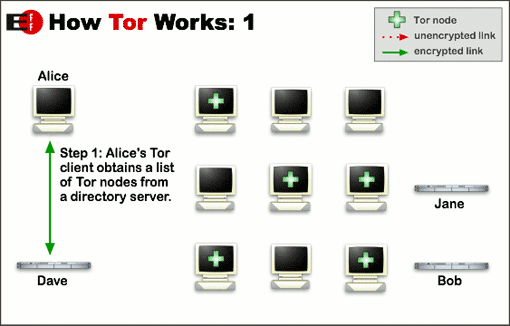
\includegraphics[width=80mm]{resources/circuit-building-1.png}
    \caption{The user's software first downloads a directory list of Tor relays. This information is later used to construct a circuit through the network.\cite{McCoy2008}\cite{TorOverview}}
\end{minipage}
\end{figure}

The second step involves choosing three unique nodes to use, establishing an encrypted connection with the first one, and then extending the circuit one hop at a time such that no single relay ever knows the complete path. Each relay can only perform one layer of decryption, so data is decrypted in an onion-like fashion as it passes through the circuit.

\begin{figure}[htbp]
\centering
\begin{minipage}{8 cm}
    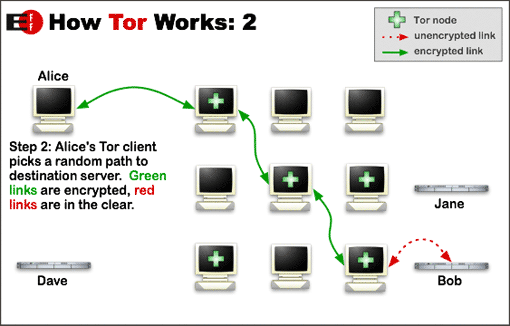
\includegraphics[width=80mm]{resources/circuit-building-2.png}
    \caption{A Tor circuit is incrementally constructed using layers of encryption. Each node has limited visibility, and no individual node knows the whole circuit.\cite{TorOverview}}
\end{minipage}
\end{figure}

The client first establishes a TLS connection with the first relay, $R_{1}$, using the relay's public key. The client then uses a single Diffie-Hellman-Merkle key exchange to negotiate $K_{1}$ which is then used to generate two symmetric keys: a forward key $K_{1,F}$ and a backwards key $K_{1,B}$. $K_{1,F}$ is used to encrypt all communication from the client to $R_{1}$ and $K_{1,B}$ is used for all replies from $R_{1}$ to the client. These keys are used conjunction with the symmetric cipher suite negotiated during the TLS handshake, thus forming an encrypted tunnel. Once this one-hop circuit has been created, the client then sends $R_{1}$ the RELAY\_EXTEND command, the address of $R_{2}$, and the client's half of the Diffie-Hellman-Merkle protocol ($ g^a mod b $) using $K_{1,F}$. $R_{1}$ performs a TLS handshake with R${2}$ and uses $R_{2}$'s public key to send $ g^a mod b $ to $R_{2}$, who replies with his half of the handshake and a hash of $K_{2}$. $R_{1}$ then forwards this to the client under $R_{1,B}$ with the RELAY\_EXTENDED command to notify the client. The client generates $K_{1,F}$ and $K_{1,B}$ from $K_{2}$, and repeats the process for $R_{3}$,\cite{Ling2012} as shown in Figure 3. The TLS/IP connections remain open, so the returned information travels back up the circuit to the end user.

\begin{figure}[htbp]
\centering
\begin{minipage}{8 cm}
    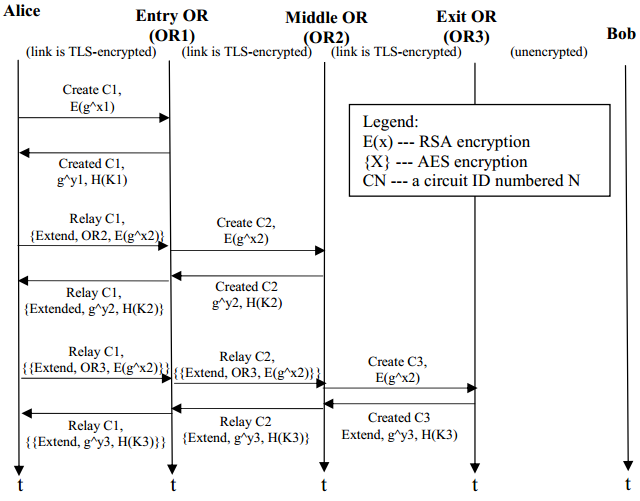
\includegraphics[width=80mm]{resources/circuit-construction.png}
    \caption{A Tor circuit is incrementally constructed using layers of encryption. Each node has limited visibility, and no individual node knows the whole circuit.\cite{TorOverview}}
\end{minipage}
\end{figure}

Following the complete establishment of a circuit, the Tor client software then offers a Secure Sockets (SOCKS) interface which multiplexes TCP traffic through Tor. At the application layer, this data is packed and padded into equally-sized Tor \textit{cells}, transmission units of 512 bytes. As each relay sees no more than one hop in the circuit, in theory neither an eavesdropper nor a compromised relay can link the connection's source, destination, and content. Tor further obfuscates user traffic by changing the circuit path every ten minutes,\cite{McCoy2008} as shown in Figure 4.

\begin{figure}[htbp]
\centering
\begin{minipage}{8 cm}
  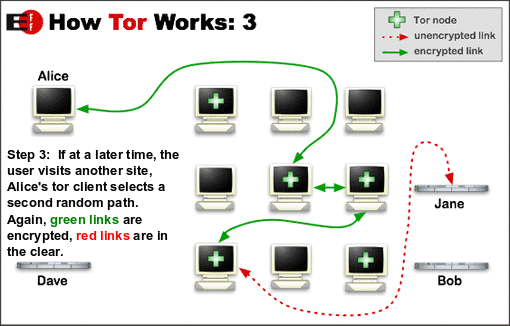
\includegraphics[width=80mm]{resources/circuit-change.png}
  \caption{A Tor circuit is changed periodically, essentially providing a new identity to the end user.\cite{TorOverview}}
\end{minipage}
\end{figure}

An encrypted connection is often established with the other client or web server, depending on whether or not the recipient supports encryption. If this is the case, even the exit node cannot see the traffic in cleartext. An outsider is therefore faced with up to four layers of TLS encryption: $K_{1,F}(K_{2,F}(K_{3,F}(K_{server}(client\ request))))$ and likewise $K_{1,B}(K_{2,B}(K_{3,B}(K_{server}(server\ reply))))$ for the returning traffic. This makes traffic analysis and cryptographic attacks very difficult.

\subsection{Encryption}

% http://security.stackexchange.com/questions/8343/what-key-exchange-mechanism-should-be-used-in-tls
% https://en.wikipedia.org/wiki/Comparison_of_TLS_implementations
% https://www.ipa.go.jp/security/rfc/RFC5246-ACJA.html

Encryption is a necessary to achieve privacy both inside and outside the Tor network. Traffic passing between nodes must be secured from outsiders to prevent adversaries from following the entire circuit. Layers of encryption also prevent compromised nodes from observing the traffic in cleartext. The exit node is especially important; encrypted connections are often established the recipient outside Tor so that the exit node cannot observe the intended message.

Within the network, nodes talk to each other via the Transport Security Layer (TLS) protocol. During circuit construction, the client incrementally performs a handshake with each relay in turn, establishing an agreement over the encryption key and specific symmetric cipher. There are several mechanisms by which this is done, most of which use the Diffie-Hellman-Merkle (DH) protocol for key exchange. The ephemeral version of DH provides perfect forward secrecy by generating a new session key for every handshake. The secret keys for DH ($a$ and $b$) are not stored, preventing attackers from decrypting prior communication even if the relay is later compromised. Authentication of communication is achieved through RSA or elliptic curve public keys, with the SHA-1 serving as the hash function for integrity verification.

Tor users typically use the Tor Browser Bundle, (TBB) a custom build of Mozilla Firefox with a focus on security and privacy. The TBB not only provides special handling of client-side scripts such as Javascript, but also offers the HTTPS Everywhere extension, which uses regular expressions to rewrite HTTP web requests into HTTPS whenever possible. Thus, if the web server is capable of handling SSL or TLS connections, HTTP communications will be encrypted to them. If this is the case, the TBB performs a TLS handshake with the web server, but the exchange happens through the Tor circuit. This provides the final layer of encryption to the outside.

In September 2013, Robert Graham of Errata Security performed a small study on what cryptography methods Tor primarily used. His exit node analyzed 22,920 incoming connections found that 89.9\% of the circuits agreed to use the Advanced Encryption Standard (AES) block cipher in cipher-block chaining (CBC) mode. This is the most common mode for AES, and allows for parallel decryption of the data blocks. The other 10.1\% of the circuits relied upon three rounds of the Data Encryption Standard (triple DES) cipher for encryption. Furthermore, 75.7\% of the circuits used elliptic-curve DH, with the remaining 22.3\% relying upon traditional RSA DH.\cite{Graham2013} Both protocols are discussed below.

\subsubsection{RSA}

RSA is an algorithm for public-key cryptography. Its security is based on the infeasibility of factoring the product of two large primes. RSA, like all other public-key cryptography algorithms, relies upon two keys: one public and the other private. The public key may be published and is used for encryption and for the verification of digital signatures. The private key is used for decryption and the generation of digital signatures. Thus, only the owner of the private key can decrypt incoming messages, and only they can digitally sign outbound messages. These properties make RSA and other public-key algorithms extremely powerful as they can provide authenticity, integrity, and privacy of communications between two parties.

However, RSA operations are computationally expensive, and RSA only provides one-way authentication and privacy. Both parties must have RSA keys in order to achieve private two-way authenticated communication. This situation is unlikely and often infeasible to implement, so RSA is used by TLS in conjunction with faster symmetric-key encryption algorithms.

Tor version 2.3.x and previous primarily rely upon TLS\_DHE for the key exchange mechanism. In this protocol, Bob replies to Alice with a dynamically-generated (ephemeral) DH key and signs this with his private RSA key. Alice can then confirm the digital signature to verify the authenticity of the communication. Thus the client can prove the authenticity of replies from Tor relays in the circuit or with the end web server.

\subsubsection{Elliptic-curve}

Elliptic Curve Cryptography (ECC) is an approach to public-key cryptography in which elliptic curves are used instead of RSA. In contrast to RSA, ECC relies upon the infeasiblity of finding the discrete logarithm of a random elliptic curve element with respect to a publicly known base point. This is known as the elliptic curve discrete logarithm problem, or ECDLP.

A smaller key size is one of the most significant benefits introduced by ECC. Current NIST recommendations state that a key size of 160 bits for ECC offers a similar level of security to 1024 bits of RSA and Diffie-Hellman-Merkle. Likewise, 224 bits for ECC is analogous to 2048 bits of RSA/DH. It should be noted that the required key sizes for ECC increases significantly slower than the key sizes for RSA/DH. Thus ECC offers more security per increase in key size than for RSA. The smaller key size also directly correlates to an increase in computational efficiency; as the bit size increases, the speed difference between RSA/DH and ECC operations grows superlinearly.\cite{CaseForECC}

Tor is currently undergoing a transition from RSA-based to elliptic-curve-based TLS. Tor 2.4.x introduced TLS\_ECDHE, which uses an elliptic-curve variant of DH and it became the preferred key exchange protocol. 2.4.x relays also offer both an RSA and elliptic curve public key for authentication purposes in TLS. The transition to ECC reduces computational demand and is believe to provide stronger security.

\subsubsection{Symmetric-key}

% http://www.isg.rhul.ac.uk/tls/
% https://community.qualys.com/blogs/securitylabs/2013/03/19/rc4-in-tls-is-broken-now-what

Once the TLS handshake and DH key exchanges complete, both parties use the generated session key and turn to symmetric-key encryption for hiding of data. Common symmetric-key algorithms include Data Encryption Standard, Advanced Encryption Standard, and RC4.

Both DES and AES are block ciphers, whereas RC4 is a stream cipher. DES, shown to be susceptible to brute-force attacks in 1998, has been replaced by triple-DES, (3DES) which itself has been succeeded by the much-stronger AES cipher. However, 3DES is still used on the web and by older Microsoft products.\cite{NIST2007}\cite{Bogdanov2011}\cite{Nikolic2009} The RC4 cipher is simple and extremely fast in software, and is now the most widely used software stream cipher, most notably in protocols such as TLS and WEP.

Robert Graham's analysis of the incoming handshakes to his exit node revealed that almost 90\% of the circuits agreed on the AES cipher, while the remainder used 3DES. For communication to web servers, RC4 remained the most popular algorithm.\cite{Graham2013}

% -------------------------------------------------------------------------------

\section{Attacks and Defenses}

Attacks from adversaries against Tor can be classified into several categories: attack on the user, attacks on their computer, attacks on the Tor network itself, attacks on the exit's connection across the Internet, and attacks on the server. Tor's developers have implemented or recommended various defenses against common attacks on each of these layers.

\subsection{Social engineering}

Human mistakes are one of the most serious threats to deanonymization, and defenses against it are outside the scope of the Tor project. While Tor users can enjoy a reasonable level of anonymity and protection against traffic analysis, use of the Tor network is useless if information about their identity and/or location is leaked to the Internet. The electronic trail they leave behind can be used to completely deanonymize them and reveal their activities. The Tor Project provides recommendations that aim to prevent users from leaking their identity, but actual defenses against this attack are generally outside the scope of Tor.

(notable examples, describe defenses)

\subsection{Malware}

Tor users can also be revealed or have their privacy compromised by their own workstations. If their computer contains spyware, backdoors, or other malicious software that can be used to identify them or their traffic, then a user may be tricked into believing that they are anonymous when in fact they are not.

(going to expand this a bit more, discuss Javascript vs NoScript, cross-site scripting attacks, TBB defenses)

\subsection{Attacks against the Tor network}

% https://blog.torproject.org/blog/improving-tors-anonymity-changing-guard-parameters

The relay chosen for the first hop in the circuit has knowledge of the user's IP address, can thus deanonymize them in that respect. Although this first relay does not know the rest of the circuit and cannot deduce the final traffic exiting Tor, the knowledge of the user's IP can be problematic if the relay is operated by an attacker. With this information, an adversary would be able to trace users or deny them entry into the Tor network.

Tor attempts to combat this through \textit{entry guards}, a feature introduced in May 2006. Directory servers mark relays as guards as both being fast (i.e. has bandwidth above the median of all other relays) and stable (i.e. averages and uptime above the median of all other relays). The Tor client software chooses three guards out of the pool and then exclusively picks from these chosen relays as the first hop of any circuit.\cite{Xin2009} The goal of this selection is to protect the end user against the ``predecessor attack'', wherein the attacker can preform end-to-end correlation and deanonymize the user if compromised nodes are chosen for the first and last hop in the circuit.\cite{Wright2004} As relays initially are only the middle hop, this approach also makes it more difficult for an attacker to add relays to the Tor network and immediately begin tracing users. As of the time of this writing, there are 4,737 relays on the Tor network, which means that the chances of a client including a compromised node in its selection pool is 4,737 choose three without replacement, or 0.06334\%.

To achieve its low-latency objective, Tor does not explicitly re-order or delay packets within the network.\cite{McCoy2008} If an adversary controls both the first hop and the final hop in the Tor circuit, then it may be possible for the attacker to perform timing attacks. To do this, the attacker would listen for incoming packets from a certain IP and simultaneously keep track of traffic flow out of the exit node. They could then use statistics to gain a reasonable correlation between the incoming and outgoing traffic. This would result in a deanonymization of the end-user and, if the connection to the web server was not encrypted, reveal their traffic. At its onset Tor was susceptible to this timing attack, but as the size and usage of the Tor network increased, the likelihood of successfully launching such a traffic analysis attack quickly became negligible.\cite{Xin2009}

\subsection{Wiretapping the exit node}

Exit nodes are valuable on the Tor network due to their necessity for the final hop of the circuit and because they are rarer than traditional relays. Exit node operators typically have to deal with ISP complaints for any nefarious Internet activities performed by the users at the other end of the circuit. Although these complaints can be largely combated by implementing a reduced exit policy, there are 912 exit notes at the time of this writing, 19.74\% of the total 4,737 relays on the Tor network. It is entirely possible than an adversay could control an exit node, giving them insight into the traffic leaving Tor. If the traffic is encrypted, the exit node could still see the DNS lookup and HTTP headers. If encryption is not implemented, all traffic would thus be available for inspection.

In September 2007, Swedish security consultant Dan Egerstad operated five exit nodes and monitored their traffic. Over the course of his experiment, he obtained the usernames and passwords for over 100 email accounts, read the correspondence from embassies in Australia, Japan, Iran, India, and Russia, along with communication between dignitaries including the Indian ambassador to China, various politicians in Hong Kong, workers in the Dalai Lama's liaison office, and several human-rights groups in Hong Kong. He also obtained sensitive spreadsheets and documents about military and political activities. Egerstad's analysis further revealed that approximately 95\% of the traffic flowing over his nodes was not encrypted.\cite{Wired2007}

An adversary could operate one or more exit nodes, as Egerstad did, or they could wiretap the exit's traffic and gain access to the traffic that way, perhaps without the knowledge of the exit operator. While the exit has no knowledge of the entire circuit and thus cannot deduce the origin of the traffic, the unencrypted traffic can be quite revealing and problematic, as Egerstad demonstrated. The primary way that Tor combats this through encryption. The Tor Browser Bundle comes with the HTTPS Everywhere, which prefers the use of HTTPS when connecting to web servers. Most email servers also support SSL/TLS, and users can also manually encrypt their documents or emails using PGP. Although Tor has no way of enforcing this final layer of encryption, it highly recommends it and places notices about this on many places on its website.

\subsection{Web server vulnerabilities}

The web server can also be a point of failure for the privacy and anonymity of the end user.

(going to expand this a bit more. Does the web server support SSL/TLS? The adversary could fake masquerade as the server)

\subsection{Cryptographic Attacks}

Although it is popular, a number of practical attacks and weaknesses have been demonstrated against its Key Scheduling Algorithm and PRNG that call into question RC4's security. In November 2013, Microsoft recommended disabling RC4 from TLS wherever possible.

\subsection{Network-layer Exploitation}

\begin{figure}[htbp]
\centering
\begin{minipage}{8 cm}
    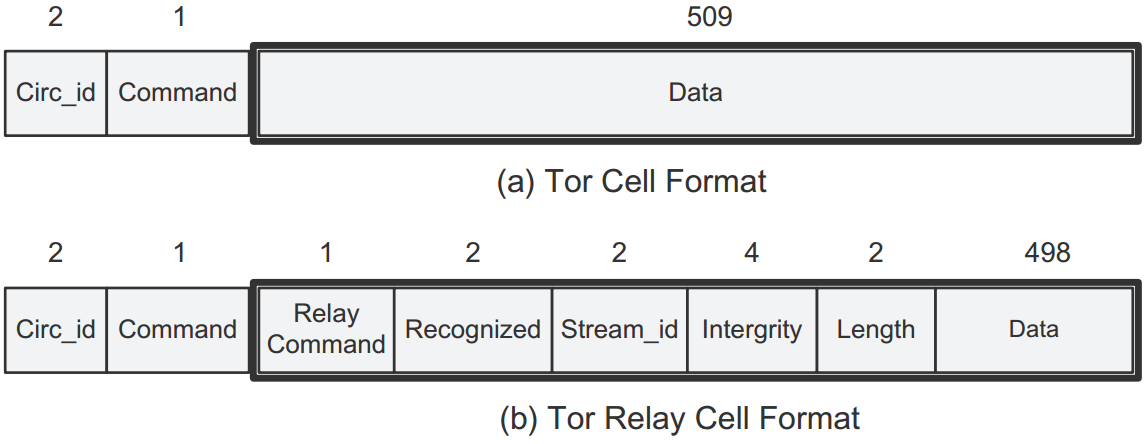
\includegraphics[width=80mm]{resources/tor-cell-format.png}
    \caption{The format of a Tor cell. The command field of a control cell (a) can be CELL\_PADDING, CELL\_CREATE, or CELL\_DESTROY, the latter two of which are used for creating a circuit to a relay. Only the 509-byte data section is encrypted in an onion-like fashion. \newline\hspace*{2em} The command field of a relay cell is CELL\_RELAY. The Relay Command header can be of numerous types, including RELAY\_BEGIN, RELAY\_DATA, RELAY\_END, RELAY\_EXTEND, and RELAY\_EXTENDED. DNS host resolution is signified by RELAY\_RESOLVE. The Recognized field is used to identify whether the cell is correctly recognized by the client or exit router. Stream\_ID is useful as multiple data streams can be multiplexed down a Tor circuit at the application layer by either the client and the exit node. The Integrity field is used to verify the integrity of the cell data, and the final Length field specifies the size of the traffic data, which may be padded.}
\end{minipage}
\end{figure}

Another potential method to de-anonymize users is through active watermarking of packets. Digital watermarks require less time deploy, often have a higher success rate, and do not require observing traffic for long periods of time. If an attacker can modify the traffic flow such that it is noticable at the other end of Tor, then it becomes easy to identify end users and correlate them with their activities.

In 2011, Zhen Ling \textit{et al} described an active watermark attack in which an attacker operates a reverse proxy and actively manipulates the size of the TCP packets transmitted to the exit node. Simultaneously, the attacker also runs a recovery method to detect the watermark on the user side. His watermark was a short sequence of 1s and 0s that could be encoded into the packet patterns. To transmit a 0, the attacker sends 498 bytes worth of web traffic to the Tor exit node, which is the exact size of the data portion of a Tor cell. Combined with the cell headers, the data packs into a single Tor cell of 512 bytes. To transmit a 1, the attacker sends 2444 bytes of data to the exit. The standard Maximum Transmission Unit (MTU) for Ethernet v2 lines is 1500 bytes and the TCP and IP headers are 20 and 32 bytes respectively, which means that a TCP packet can carry at most 1448 bytes of data. As the 2444 bytes from the attacker exceeds the MTU, two TCP packets are needed, one with a 1448-byte payload and the other with a 996-byte payload. The first TCP packet is received by the relay and is packed into three equally-sized cells, with padding added to the 452 bytes of the third cell. The second TCP packet becomes two cells of 498 bytes each, and thus the 2444 bytes becomes five Tor cells. Then these cells are processed, encoded as TCP packets, and retransmitted to the next relay. However, due to the design of cell queuing algorithms, TCP retransmission, and MTU restrictions, the two TCP packets may be split and combined into Tor cells in up to five different ways, each leaving a discernible packet signature. The attacker can then monitor the traffic near the client, examining the packet patterns generated by the attack. If the embedded signal is found, then it is quite likely that the traffic flows are correlated. In their tests, Zhen Ling \textit{et al} achieved a detection rate of nearly 90\%, with a false positive rate of less than 4\%, concluding that such an attack could degrade anonymity if applied in practice.\cite{Ling2011}



\section{Adversaries}

Tor is designed to counter traffic analysis and circumvent censorship, so naturally most adversaries against Tor are those who wish to enforce Internet censorship or watch the electronic activities of certain groups and organizations. Such adversaries can range from a small number of individuals to whole branches within national governments.

\subsection{China}

One of the most famous examples of Internet censorship is the Great Firewall of China, a project launched in late 2003 which aims to prohibit individuals from using the Internet for activities which are not approved by the Chinese government. The Chinese Ministry of Public Security maintains the most sophisticated content-filtering regime in the world and actively engages in DNS cache poisoning, IP/URL blocking, and packet filtering.

Chinese citizens have increasingly grown increative in their attempts to \textit{fanqiang}, or ``climb the wall''. The Chinese government responds by actively blocking VPNs, proxies, and Tor relays. Despite these efforts, users are able to bypass the firewall via \textit{Tor bridges}, which act as the first hop into the Tor network. The list of bridges is not publicly published, making them difficult to blacklist. The Great Firewall of China attempts to dynamically block these bridges by detecting the Tor TLS handshake, probing the target bridge, and then blocking it if it responds with the Tor protocol. However, users can still easily gain access to Tor (and thus the rest of the Internet) by the use of Obfsproxy. Bridges that are wrapped with the Obfsproxy tool disguise their TLS handshake so that it looks like normal HTTP traffic and otherwise carries no discernible byte characteristics to the outside world, making Obfsproxy bridges nearly impossible to detect.\cite{Anderson2013}

\subsection{NSA}

Earlier this year, Edward Snowden revealed that the United States National Security Agency (NSA) has been attempting to penetrate the Tor network and de-anonymize its users, but with little success. In a June 2012 PowerPoint presentation titled ``Tor Stinks'', the NSA stated that ``with manual analysis we can de-anonymize a \textit{very small fraction} of Tor users'' but admitted that they have had no success in identifying a user on demand, and that they will never be able to de-anonymize all Tor users all the time. However, they had performed research on a variety of attacks against Tor. Their purpose was reveal ``terrorists'' and other individuals of interest to the United States.

Their documents revealed that as of 2012 they had access to very few nodes and that their goal is to control more, as they had only seen negligible success with circuit construction attacks. Further notes showed that they have had little success with timing attacks, and that they had put no effort towards revealing hidden services. While the NSA has Computer Network Exploitation (CNE) tools at their disposal for Windows, OS X, and Linux, as of 2012 CNE has been unsuccessful against the Tor Browser Bundle. If CNE exploits were possible, the NSA was considering the implications of attempting to direct the client to prefer NSA-controlled exit nodes, a private Tor network run by the NSA, or to reveal the client's IP by contacting an NSA web server directly. They were working on implementing this shaping attack. The NSA documents also showed that it was likely not legally or technically possible for them to exploit existing nodes, though they were considering exploiting web servers to make web surfing more difficult for Tor users. Considering psychological attacks, the authors concluded that Tor contained a critical mass of users, and that attempting to scare the public away from Tor could be counterproductive.\cite{GuardianTorStinks}

The Tor developers responded to these and other related articles, saying ``the good news is that they went for a browser exploit, meaning there's no indication they can break the Tor protocol or do traffic analysis on the Tor network. Infecting the laptop, phone, or desktop is still the easiest way to learn about the human behind the keyboard.'' and ``if you attack too many users, somebody's going to notice. So even if the NSA aims to surveil everyone, everywhere, they have to be a lot more selective about which Tor users they spy on. Just using Tor isn't enough to keep you safe in all cases.''. The developers also commented that the described attacks seemed ``relatively basic'' and ``out-of-date'', saying ``we still have a lot of work to do to make Tor both safe and usable, but we don't have any new work based on these slides''.\cite{TorBlogGuardian}

\subsection{FBI}

One of the most famous attacks against Tor by the FBI was the successful finding and subsequent takedown of the Silk Road, a black market operating purely inside the Tor network as a hidden service. The Silk Road, sometimes called the ``eBay of illegal drugs'', first went online in February 2011, and remained covertly in use for two years later before Australian police discovered clues to its existence. The service could not be accessed from the traditional Internet, and, like other hidden services in the ``darknet'', was only available through the Tor network. On October 2, 2013, the FBI shut down the Silk Road and arrested the alleged owner, Ross Ulbricht in San Fransisco. Ulbricht mistakenly revealed his primary email address on a forum and later exposed his real IP by posing a question related to Silk Road on StackOverflow.com without using Tor. These clues then led to his arrest.

The Tor Project responded to the Silk Road takedown with an analysis of the Tor network, saying ``So far, nothing about this case makes us think that there are new ways to compromise Tor (the software or the network). The FBI says that their suspect made mistakes in operational security, and was found through actual detective work.'' further saying that they found no evidence that the FBI broke into the webserver. They also reinforced their recommendations against providing personal information online.\cite{TorBlogSilkRoad}

\section{Analysis}

(going to expand this a bit more and devote the couple pages to this section. I've got IEEE citations like \cite{Xin2009}, \cite{Ling2011}, and \cite{Ling2012} that should be very helpful in demonstrating some weaknesses of Tor

Bauer and McCoy, \textit{et al}, described a low-resource routing attack against the Tor network.\cite{Bauer2007}



\section{Conclusion}

Tor provides an anonymity and privacy layer by relaying end-user traffic through a circuit consisting of three randomized relays around the world. Traffic is encrypted with the session keys of each relay and then decrypted in an onion-like fashion as it passes through the circuit. No single relay knows both the source IP and its destination, so even single compromised relays are unable to correlate end users with their activities. This makes Tor much more resilient to adversaries than proxies or VPNs. For this reason, it is one of the most popular and secure tools to use against network surveillance, traffic analysis, and Internet censorship. Tor has been attacked by various organizations, agencies, and governments in an attempt to watch users, root out their identities, or restrict their access to information. Although its main adversaries are well-resourced, Tor's routing and cryptography protocols have made it very difficult for outsiders to penetrate its defenses.

However, Tor is not impenetrable. By far the most significant threat to Internet anonymity is carelessness: a user may publish enough electronic clues that point to their real-life identity. By design, Tor cannot defend against this. The most effective attacks against Tor itself have used exploits in the Tor Browser Bundle, Javascript, or the host operating system. These indirect attacks have been used in the past to successfully de-anonymize a few of its users. In other cases, traditional detective work has been used to take down hidden services inside the Tor network. However, in general the Tor routing protocol has proven fairly secure, with only a handful of theoretical attacks published and tested by researchers in the field. As Tor's documentation suggests, it is not a foolproof solution for online anonymity, and users must still be careful with their information.

Tor's developers and the open-source community continue to update the software with improved cryptography and preemptive security patches. This makes exploiting Tor a continual and difficult race against global open-source development, certainly a challenge for even well-resource adversaries. Indeed, an NSA appraisal released by the Guardian in October 2013 characterizes Tor as ``still the king of high secure, low latency Internet anonymity'' and that ``there are no contenders for the throne in waiting''. Tor's future looks bright.

% -----------------------------------------------------------------------------

% https://en.wikibooks.org/wiki/LaTeX/Bibliography_Management
\begin{thebibliography}{9}

% http://freehaven.net/anonbib/#Wright:2004
\bibitem{Wright2004}
  Matthew Wright, Micah Adler, Brian Neil Levine, and Clay Shields
  \emph{The Predecessor Attack: An Analysis of a Threat to Anonymous Communications Systems}.
  ACM Transactions on Information and System Security (TISSEC) 4(7), November 2004, pages 489-522

% http://ieeexplore.ieee.org/stamp/stamp.jsp?tp=&arnumber=5636000&tag=1
\bibitem{Chaabane2007}
  Abdelberi Chaabane, Pere Manils, Mohamed Ali Kaafar
  \emph{Digging into Anonymous Traffic: a deep analysis of the Tor anonymizing network}.
  IEEE, 2010

% http://www.wired.com/politics/security/news/2007/09/embassy_hacks
% http://www.wired.com/threatlevel/2007/08/embassy-e-mail/
\bibitem{Wired2007}
  Kim Zetter
  \emph{Rogue Nodes Turn Tor Anonymizer Into Eavesdropper's Paradise}
  Wired, 2007

% http://csrc.nist.gov/publications/nistpubs/800-57/sp800-57-Part1-revised2_Mar08-2007.pdf
\bibitem{NIST2007}
  Elaine Barker, William Barker, William Burr, William Polk, and Miles Smid
  \emph{Recommendation for Key Management, Part 1: General (Revised)}
  National Institute of Standards and Technology, March 2007

% http://delivery.acm.org/10.1145/1320000/1314336/p11-bauer.pdf?ip=129.123.212.2&id=1314336&acc=ACTIVE%20SERVICE&key=C2716FEBFA981EF14CED21A2601DAAECFD63F9AFA4F38248&CFID=375634674&CFTOKEN=21383502&__acm__=1383519744_1cd525050cafbe9ffe083b269ff783d9
\bibitem{Bauer2007}
  Kevin Bauer, Damon McCoy, Dirk Grunwald, Tadayoshi Kohno, Douglas Sicker
  \emph{Low-resource routing attacks against tor}.
  ACM, 2007

% http://homes.cs.washington.edu/~yoshi/papers/Tor/PETS2008_37.pdf
\bibitem{McCoy2008}
  Damon McCoy, Kevin Bauer, Dirk Grunwald, Tadayoshi Kohno, Douglas Sicker,
  \emph{Shining Light in Dark Places: Understanding the Tor Network}.
  Department of Computer Science and Engineering,
  University of Washington, Seattle, WA 98195-2969,
  2008.

% http://link.springer.com/chapter/10.1007%2F978-3-642-03356-8_14
\bibitem{Nikolic2009}
  Nikolić, Ivica
  \emph{Distinguisher and Related-Key Attack on the Full AES-256}
  Advances in Cryptology, 2009

% http://ieeexplore.ieee.org/stamp/stamp.jsp?tp=&arnumber=4797313
\bibitem{Xin2009}
  Liu Xin, Wang Neng
  \emph{Design Improvement for Tor Against Low-Cost Traffic Attack and Low-Resource Routing Attack}
  2009 International Conference on Communications and Mobile Computing

% http://www.nsa.gov/business/programs/elliptic_curve.shtml
\bibitem{CaseForECC}
  National Security Agency
  \emph{The Case for Elliptic Curve Cryptography}.
  NSA, 2009

% https://research.microsoft.com/en-us/projects/cryptanalysis/aesbc.pdf
\bibitem{Bogdanov2011}
  Andrey Bogdanov, Dmitry Khovratovich, and Christian Rechberger
  \emph{Biclique Cryptanalysis of the Full AES}
  Microsoft Research Redmond, 2011

% http://ieeexplore.ieee.org/xpls/abs_all.jsp?arnumber=5962653
\bibitem{Ling2011}
  Zhen Ling
  \emph{Equal-Sized Cells Mean Equal-Sized Packets in Tor?}
  IEEE International Conference on Communications, 2011

% http://ac.els-cdn.com/S1389128612003799/1-s2.0-S1389128612003799-main.pdf?_tid=c6751d5e-5009-11e3-9ab2-00000aab0f26&acdnat=1384749046_78b8af8ba2cb2c0a2672840e0c7c5da1
\bibitem{Ling2012}
  Zhen Ling, Junzhou Luo, Wei Yu, Xinwen Fuc, Weijia Jia, Wei Zhao
  \emph{Protocol-level attacks against Tor}
  Computer Networks, 2012

% http://blog.erratasec.com/2013/09/tor-is-still-dhe-1024-nsa-crackable.html
% http://thehackernews.com/2013/09/NSA-can-crack-TOR-Encryptio-Snowden-files-.html
\bibitem{Graham2013}
  Robert Graham
  \emph{Tor is still DHE 1024 (NSA crackable)}.
  Errata Security, 2013

% http://queue.acm.org/detail.cfm?id=2405036
\bibitem{Anderson2013}
  Daniel Anderson
  \emph{Splinternet Behind the Great Firewall of China: The Fight Against GFW}.
  Association for Computing Machinery (ACM), Vol. 10, No. 11 (29 November 2012), doi:10.1145/2390756.2405036

% https://blog.torproject.org/blog/tor-and-silk-road-takedown
\bibitem{TorBlogSilkRoad}
  arma
  \emph{Tor and the Silk Road takedown}
  The Tor Blog, 2 October 2013

\bibitem{GuardianTorStinks}
  The Guardian
  \emph{'Tor Stinks' presentation}
  The Guardian, 4 October 2013

\bibitem{TorBlogGuardian}
  Roger Dingledine
  \emph{Yes, we know about the Guardian article}
  Tor Project Blog, 4 October 2013

% https://www.torproject.org/about/overview.html.en
\bibitem{TorOverview}
  Overview of Tor

\end{thebibliography}

\end{document}
